\documentclass[10pt, conference]{lib/IEEEtran}

\usepackage{graphicx}
\usepackage{color}
\usepackage{epstopdf}
\usepackage{amsmath}
\usepackage{float}
\usepackage[font=small]{caption}

\begin{document}

\title{Performance Analysis of TCP Variants}

\author{\IEEEauthorblockN{Zhemin Mi}
\IEEEauthorblockA{College of Engineering\\
Northeastern University, MA, 02115\\
Email: mi.z@husky.neu.edu\\}
\and
\IEEEauthorblockN{Binbin Lu}
\IEEEauthorblockA{College of Engineering\\
Northeastern University, MA, 02115\\
Email: lu.b@husky.neu.edu\\}
}
\maketitle


\begin{abstract}
This paper simulated and analyzes the performance between different TCP variants on a simple network topology with a tool called NS-2. The key comparision factors this looking for between TCP variants are latency, drop rate, throughput and fairness. Multiple experiments were simulated against Tahoe, Reno, NewReno and Vegas. Finally, this paper investigated the queuing influences with TCP Reno and SACK.
\end{abstract}


\section{Introduction}
The original design of the Transmission Control Protocol (TCP) worked 
reliably, but was unable to provide acceptable performance in large 
and congested networks. Several TCP variants have been proposed since 
then (TCP Tahoe, Reno, NewReno, Vegas, BIC, CUBIC, SACK, and others) 
with mechanisms to control and avoid congestion. In this paper, we 
performed a couple of simulations using NS-2 to compare the 
performance of TCP Tahoe, Reno, NewReno and Vegas under same topology. 
In experiment1, we investigated the throughput, drop rate and latency 
under a certain congestion, which is simulated by a UPD based Constant 
Bit Rate (CBR); In experiment2, this paper compares the fairness 
between Reno/Reno, NewReno/Reno, Vegas/Vegas and NewReno/Vegas under 
simular variants congestion as experiment1; In experiment3, we learned 
the impact of queuing disciplines, DropTail and Random Early Drop (RED)
, on TCP Reno and SACK.


\section{Experiment 1: TCP Performance Under Congestion}
The network topology and flow setup of experiment 1 is as figure~\ref{fig:exp1_tpg}.
\begin{figure}[!htb]
    \centering
    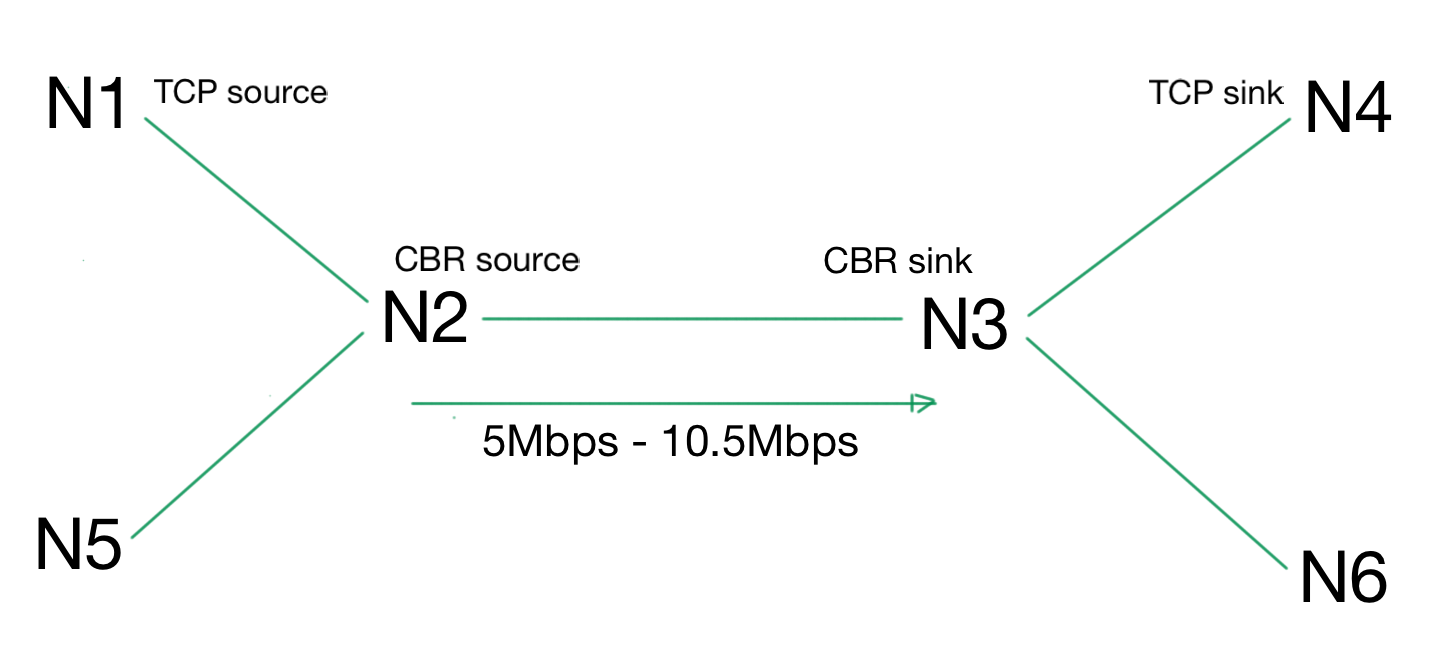
\includegraphics[width=0.8\linewidth]{images/top_exp1.png}
    \caption{Experiment 1 Network Topology}
    \label{fig:exp1_tpg}
\end{figure}
The methodology of this experiment is simple and straightforward: we 
build the topology first, then start the CBR flow from N2 to N3 and 
TCP flow from N1 to N4 later. In each separate simulation, the CBR rate
is steady and from the range of 5Mbps and 10.5Mbps, TCP flow is one of 
TCP Tahoe, Reno, NewReno and Vegas. The CBR rate increases 0.5Mbps 
every time and we run simulations for each TCP variant against all 
rates. For a single TCP variant and a single CBR rate, about 100 
simulations were performed by slightly veried start time of TCP flow. 
We did this to get the average and standard deviation of each result 
for later t-test, to make sure the difference were statistically 
different from each other, which means the protocol caused the 
difference rather than noise or randomness. 

Because CBR has no flow control algorithm, the increase of sending 
rate will gradually fill the pipe between N2 and N3, which will cause 
congestion in the TCP flow. Differenct TCP variants have different 
congestion control algorithms, but they all should slow down the 
sending rate to coordinate with the situation. Also, congestion will 
increase the latency and packet drop rate of TCP flow. We can verify each of them in experiment1.

\subsection{Throughput}
After running the NS-2 simulation tool. a detailed simulation results 
contain all events (CBR and TCP) will be generated. We calculated the
 throughput by filtering the ACK events in N1. Everytime we receive an
 un-duplicate ACK, we know a packet has been successfully delivered. 
 The simulation result is shown in figure~\ref{fig:exp1_thp}.
\begin{figure}[!htb]
    \centering
    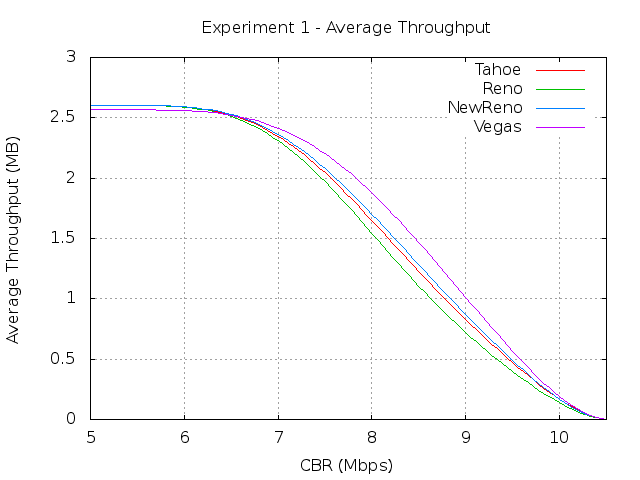
\includegraphics[width=1.0\linewidth]{plot/exp1-thp.png}
    \caption{Throughput of TCP variants}
    \label{fig:exp1_thp}
\end{figure}
For low CBR rate (e.g. CBR$ \le 6.5$Mbps), the througput of all four TCP 
variants are steady and about in the same value, with Vegas having a 
slightly lower throughput than the others. As CBR rate continues 
increase, all four TCP variants start to suffer the congestion. It is 
clearly shows that Vegas performs best in average througput, and Reno
performs the worst. The reason behind this is that Vegas is able to 
detect the congestion earlier than other variants by seeing the 
increasing Round Travel Time (RTT) values. In this way, Vegas is more 
likely to send more data while the others have to wait for timeouts or 
duplicate ACKs. But under a good network, Vegas is more senstive and 
conducts more congestion control, which makes it has lower throughput 
than others.

\subsection{Packets Drop Rate}
In the generated trace file by NS-2, drop packets at each node are 
labored with ``d'' sign. However, packets can be lost in either nodes 
or links, so we decide to calculate the lost packet by our own. We 
set a counter TOTAL-PACKET for sent packet at N1, and another counter 
EFFECTIVE-ACK for effecitve ACK (un-duplicate ACK). This way, the drop 
can be described in figure~\ref{fig:exp1_drop}.
\begin{figure}[!htb]
    \centering
    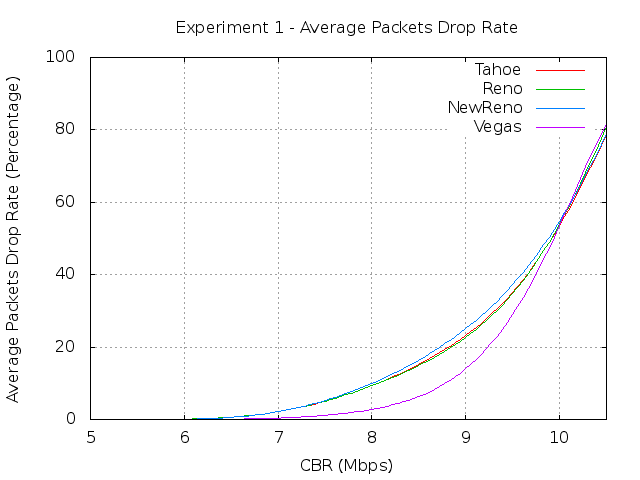
\includegraphics[width=1.0\linewidth]{plot/exp1-dr.png}
    \caption{Packets Drop Rate of TCP variants}
    \label{fig:exp1_drop}
\end{figure}
When CBR rate is below 6Mbps, no packet dropped for all four TCP 
variants. Clearly, Vegas performs better than the other three variants 
again, for two reasons. Firstly, TCP Tahoe, Reno and NewReno start to 
have dropped packets earlier than Vegas; and secondly, Vegas has 
relatively lower drop rate under all congestion conditions. Though 
Vegas has a little higher drop rate when CBR rate is bigger than 
10Mbps, it cannot deny the better ``most-conditions'' performance of 
Vegas.


\subsection{Latency}
There is no clear information in the trace file about latency, so we 
have to calculate it by our own based on the RTT. We used an array of 
floats $sentPacket$ to keep track of the sent time of each packet. 
Noticed that:
\begin{center}
    $T_{avg\_latency} = \dfrac{\sum_{i = 0}^{n - 1} (T_{ack}^i - T_{send}^i)}{sentPackets.size()}$
\end{center}
we only need another counter $totalTime$ to calculate the total transmitted time 
for later use.
Initially, all entries were set to $-1$. Everytime we detected a 
``enqueue'' at N1, we set the coressponding entry (same as packet seq 
number) to current time. Whenever we receive an valid ACK, the RTT for 
this packet was added to $totalTime$, and corresponding entry in 
$sentPackets$ is set back to -1. 
\begin{enumerate}
    \item For retransmitted packet, the sent time is the time when it firstly sent out.
    \item If we receive a ACK with corresponding entry value is -1, either it is a duplicate ACK, or an error. In both cases, we ignore the ACK.
\end{enumerate}
When the TCP flow stops, we can calculate the average latency with:
\begin{center}
    $T_{avg\_latency} = \dfrac{totalTime}{sentPackets.size()}$
\end{center}
The average latencies for the four TCP variants are showed in figure~\ref{fig:exp1_lt}
\begin{figure}[!htb]
    \centering
    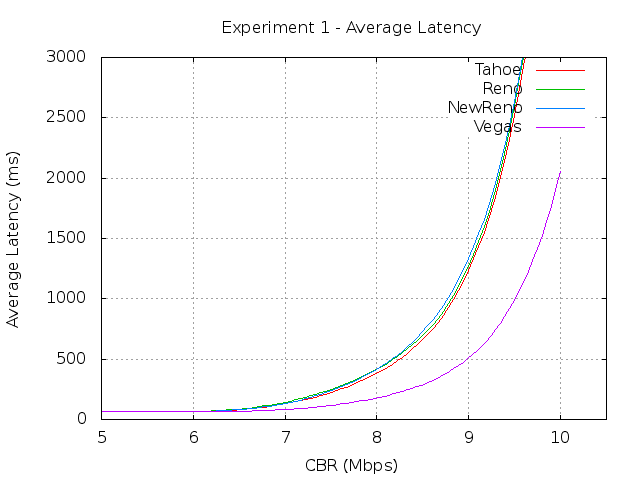
\includegraphics[width=1.0\linewidth]{plot/exp1-lt.png}
    \caption{Average Latency of TCP variants}
    \label{fig:exp1_lt}
\end{figure}
The results is similar to the other two: At a fairly low CBR rate 
(e.g. CBR rate$ \le 6$Mbps), all TCP variants performs well, the 
average latency is almost the same as optimal (60ms). As CBR rate 
continues increase, all TCP variants start to suffer longer delay, 
while Vegas has much lower latency than the other three. At 10Mbps 
CBR rate, Vegas is the only one still ``survives'', all other variants
are having too long latency, which means the packets are not likely 
delivered.

\subsection{T-Test}
The above three results show that there are differences in performance 
those four TCP variants. But we need to make sure it is caused by the
TCP protocols themselves, not by noise or randomness. Since we run the 
tests agains each variant at a certain CBR rate for 100 times, we can
perform the T-Test by using the mean and standard deviation. 
\begin{center}
    $t = \dfrac{\bar{x}_T -\bar{x}_C}{\sqrt{\frac{Var_T}{n_T} + \frac{Var_C}{n_C}}}$
\end{center}
The bigger the t is, the more likely that the difference between group T and group C are confidential. And figure~\ref{fig:exp1_t_test}
\begin{figure}[!htb]
    \centering
    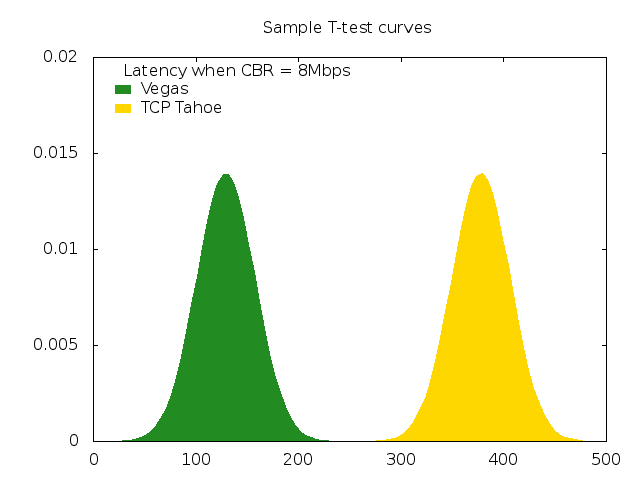
\includegraphics[width=1.0\linewidth]{plot/exp1-t-test.png}
    \caption{Sample T-test figure}
    \label{fig:exp1_t_test}
\end{figure}
is one of the t-test results. Other comparisions show similar results.
Clearly, it is due to the implementation of Vegas rather than noise 
that makes it better than other three variants.


In experiment1, we see that under a non-congested network, all four TCP
variants perform fairly the same, with low latency, good throughput and
zero drop rate. As the congestion increases, Vegas stands out in all 
three factors. However, we can still not confirm that Vegas is the best
TCP implementation of all four, because experiment 1 runs in a simple
topology. It requires a more complicated environment to confirm on that.




\section{Experiment 2: Fairness Between TCP Variants}


\subsection{Reno/Reno}


\subsection{NewReno/Reno}


\subsection{Vegas/Vegas}


\subsection{NewReno/Vegas}



\section{Experiment 3: Influence of Queuing}


\subsection{Average Bandwidth}


\subsection{Average Latency}


\section{Conclusion}
In this paper, we simulate different TCP variants with NS-2 and analyze the performance of them based on throughput, packets 
drop rate and latency. We also investigate the influence of queuing disciplines to different variants. From the 3 experiments, 
we can conclude that:
\begin{enumerate}
    \item Vegas TCP performs comparatively better than Tahoe, Reno and NewReno TCP.
    \item Same TCP variants are usually fair to each other in the same network, while different variants might suppress the \
co-existing ones.
    \item RED works well with SACK TCP, which provides low-latency and more stable transmission.
\end{enumerate}

\begin{thebibliography}{1}

\bibitem{tcp:sim}
Kevin Fall and Sally Floyd, \emph{Simulation-based Comparisons of Tahoe, Reno, and SACK TCP}.

\bibitem{tcp:ns2g}
Eitan Altman and Tania Jimenez, \emph{NS Simulator for beginners}, Lecture notes. \hskip 1em plus
0.5em minus 0.4em\relax Univ. de Los Andes, Merida, Veneuela and ESSI, Sophia-Antipolis, France: 2003.

\bibitem{tcp:plot}
Thomas Williams \& Colin Kelley, \emph{gnuplot 4.6, An Interactive Plotting Program}, 4.6.5~ed. 2014.

\bibitem{tcp:vegas}
Wikipedia, \emph{TCP Vegas}, http://en.wikipedia.org/wiki/TCP\_Vegas

\end{thebibliography}

\end{document}
